\documentclass[eric_thesis.tex]{subfiles}
\begin{document}

\chapter{Methods}

\section{Corpus: WMT11}

For training, I used the English WMT11 corpus. This is a training set collected 
for an academic competition at the sixth workshop on statistical machine 
translation. It is composed of minutes of the European parliament, news 
commentary, and news articles collected by the common crawl in the years 
2007-2011\footnote{http://www.statmt.org/wmt11/}. The European parliamentary 
minutes are in readable order. The news articles have been broken into sentences 
and those sentences included in random order\footnote{I have not read the 
rationale for this, but I believe that it was done to preserve intellectual 
property rights.}. All of the WMT11 corpus is broken into single sentence lines. 
Enclitics have been separated so ``don't'' is written as two words 
``don'\phantom{}'' and the single letter ``t''.

I chose to use the WMT11 corpus because it was both large (several billion 
words) and had already been used with the skip-gram model in 
\citep{Mikolov2013a}. Additionally, it had been originally 
compiled for a competition, this assured that much preprocessing had already 
been done.

\section{Preprocessing}

Despite some preprocessing having been done, as is customary in natural language 
processing, I still needed to do additional preprocessing to normalize the data 
for my purposes.

\subsection{Filter angle tags}

The first step I took was to remove spurious HTML and SGML tags that had been 
accidentally left in the data by the common crawl acquisition software. Most of 
the data is plain text. However, sometimes the software downloading the news 
stories did not parse the HTML correctly or the source material had erroneous 
HTML that confused the parsing software. Thus the plain text files were 
corrupted by portions surrounded by angle brackets like <P>. There were also 
stock-ticker symbols and other miscellaneous garbage included. These symbols 
would show up as words, but they are not English words and, being remnants of 
the download algorithms, are used inconsistently. To remove this digital 
flotsam, I wrote the script \filename{filter\_angle\_tags.pl} listed in 
Appendix \ref{app:filterangletags}.

I developed the script by first listing all the unique strings that began with 
< and ended with >, call each of these a tag. The function of some tags was 
obvious. For example, some were part of HTML. For each non-obvious tag, I found 
it in the corpus to determine its use from context. Then I appended it to a 
list of regular expressions to filter from the input before listing the tags. 
These filtered tags were grouped into two parts, ones O wanted to keep and ones 
I did not. When the output list was empty, I knew I had a regular expression 
covering every tag in the corpus. Then, finally, I transformed the regular 
expressions I wanted to remove into a script that would pass through only those 
regular expressions called \filename{check\_angle\_filter.pl} and created the 
\filename{filter\_angle\_tags.pl} program to remove that same group of regular 
expressions. I considered my work complete when the filtered corpus came up 
empty after being passed through \filename{check\_angle\_filter.pl}.

\subsection{Part-of-speech tagging}

An important limitation of vector based lexical semantics is its way of dealing 
with polysemy (absent mitigation techniques such as those in \citep{Erk2012}). 
Since each word gets only one meaning vector, if the 
word has more than one meaning, its associated vector is some sort of compromise 
between all of the meanings used. In the case of personality words, polysemy is 
very common. For example, consider the word ``kind''. If used in the utterance, 
``What a jerk? Of course, John is kind.'', kind carries the meaning you expect 
on a personality survey. But if used in ``What course? John is kind of a jerk.'' 
it forms part of an adverbial phrase indicating an incomplete matching to a 
description. And if used in ``What? Jerk John is a kind of course.'', kind is a 
noun that is a synonym of species. Fully distinguishing the uses is a 
significant task. However, just marking the part of speech deals with a great 
deal of the polysemy. In the example above, only the adjective is a genuine 
personality word. 

Part of speech marking misses some subtle distinctions, such as when someone 
says, ``If <person> would be so kind.'' (a common phrase in the parliamentary 
notes). However, it is very good at broader meaning differentiation. I looked 
at the 438 words used in \citep{Saucler1996}. In 
the vast majority of cases, WordNet had only one definition that had to do with 
personality and that definition was distinguished from the others by determining 
whether the part-of-speech was an adjective or not. For 6 words (cunning, 
daring, faultfinding, quiet, self-pitying, and understanding) both the adjective 
and non-adjective categories had a personality meaning. So, being an adjective 
correctly distinguished personality word semantics 98.6\% of the time.

After consulting with Dr.\ Katrin Erk, \todo{ref private communication with Dr. 
Erk} I used TreeTagger \todo{ref tree tagger paper} as my basic part-of-speech 
tagging engine. Because TreeTagger must load all sentences to be tagged into 
memory, it cannot deal with the entire corpus at once. So, I split the corpus 
into 14 files of 10,000,000 lines each (the last being smaller). TreeTagger 
(using the \filename{tree-tagger-english-utf8} script) processed these into 14 
files which had a single tagged symbol on each line. The splitting and tagging 
process was automated by my \filename{tag\_corpus.sh} script included in 
Appendix \ref{app:tagcorpus}.

\subsection{Reassemble corpus}

The 14 files were not in the single-sentence-per-line format needed by my model 
generation software. So, I wrote another script (\filename{reassemble\_tags.pl} 
Appendix \ref{app:reassembletags}) which took the 14 files, used the sentence 
ending tags to detect line ends and output only the original words except in the 
case of adjectives. Adjectives were output with an underscore and the tag JJ 
(which is the tag for an adjective used in the Penn Treebank \todo{ref penn 
treebank paper and paper giving the penn treebank tags if it is different}). So 
the word ``kind'' was output as ``kind\_JJ'' if it was an adjective.

Late in the research, I realized that \filename{reassemble\_tags.pl} did not 
put a newline at the end of the last sentence in its input file. Thus when the 
files were concatenated into the adjective-tagged corpus file, the 13 sentences 
ending the first 13 input files were concatenated with the 13 sentences starting 
the last 13 input files. Since this only affected 26 sentences out of more than 
1 billion, I decided it would not have a significant effect on the results. 
However, the version of \filename{reassemble\_tags.pl} in Appendix 
\ref{app:reassembletags} has this error corrected.

\subsection{Case folding}

For most words in English, capitalization does not affect their meaning very 
much. Much capitalization is just a marker of ``first word in the sentence.'' 
So, it is better to convert all words to lower-case. After reassembling the 
corpus, I converted all upper-case letters to lower-case. I did not convert at 
the beginning of preprocessing because capitalization is an important clue for 
part-of-speech tagging.

In a test run, I did not convert to lower-case. When I analyzed the resulting 
word-vectors, the most important component was capital versus lower-case. This 
is reasonable because the structure of the beginning of an English sentence is 
different from the structure of the rest of the sentence. For example, the 
beginning is usually the subject of the sentence. Thus, different words will 
appear at the beginning than at the end, and since capitalization frequently 
signals the beginning of the sentence, words in the subject are more likely. 
However, for the kind of meaning I want, whether a word begins a sentence is 
surplus information. So, I removed capitalization to suppress this kind of 
noise.

A disadvantage of case-folding is that some information is lost. For example: 
God and god become intermixed and Jimmy (noun) and jimmy (verb) are 
undistinguished. Almost the entire problem could be mitigated by including 
markers for proper nouns. However, it did not seem to be causing much problem, 
so I left that for later work.

\section{Number of Vector Dimensions}

Once I had the preprocessing done, the next step was to choose the number of 
dimensions in the vectors. The the vector dimensionality is an important 
parameter for any vector-based lexical semantics algorithm. For LSA, the number 
of vectors has a curvilinear relationship to meaning captured. In \todo{ref 
landauer and dumais 1987 see also handbook of LSA p.59}, performance on the 
synonym section of the TOEFL \todo{ref toefl} increased with number of 
dimensions up to about 300 and then decreased as more dimensions were added. In 
my case, I chose 800 dimensions because that was the best number of dimensions 
found for converting English to the similar language Spanish \todo{ref skip-gram 
translation paper} on the assumption that sufficient meaning to convert between 
those two languages would also be sufficient for capturing the most important 
personality dimensions.

\section{Create vectors and select words to PCA}

The number of vectors dimensions forced another trade-off. The machine available
for processing had only 8 GB of RAM. Thus, at 800 dimensions per vector, it 
could hold vectors for only 450,000 (after other overhead) since both the 
gensim and word2vec software keep the word vectors in RAM during training. 
I modified the gensim software to increase its frequency cut-off until it had removed enough
vectors so that the table fit in main memory. Thus, all words with less than 
23 appearances in the corpus were removed, leaving 449,790 different words in
the vocabulary.

Number of dimensions in hand, I generated the meaning vectors using the 
skip-gram implementation in gensim. \todo{ref gensim} Then I selected the 
meaning vectors (model.syn0) for my wordlists from the generated model using 
the script included as \filename{extract\_vectors.py} from 
\ref{app:extractvectors}. The lists of words were taken from three sets of 
personality words. 

\subsection{101 word list}

The first, containing 101 words was taken from the list of 100 words in the 
paper \citep{Goldberg1990}. To this, I added the variant spelling ``extroverted'' 
because the spelling ``extaverted'', which was in the original list, did not 
appear in the WMT11 corpus. To match the words in the tagged corpus, all of the 
words had the characters ``\_jj'' appended because the list was intended as a 
list of adjectives and JJ is the standard suffix for adjective used in the Penn 
Treebank \todo{ref cite penn treebank} and thus is the suffix used by my 
part-of-speech tagging software.

\subsection{438 word list}

The second set had 438 words and was 
taken from \citep{Saucler1996}\footnote{This paper is what I have down as 
the source for this list. However, on inspection, it has 435 words not either
439 or 438. It also lacks the word cunning twice. Thus, I believe it is the 
wrong paper. However, I reference it because it is the closest thing I have
to the correct one.}. There were 439 
entries in the list in \citep{Saucler1996}, however, the word ``cunning'' 
appeared twice. Because there were some words in the 101 word list that were 
absent in the 438 words list, I did another run with the two lists combined.

\subsection{Norman's 2797 word list}

The third set had 2797 words\footnote{The paper is entitled 2800 words, but 
mentions
that three of the words are unintentional duplicates leaving 2797 words.}
taken from \citep{Norman1967}. This paper
was available only as data automatically recognized from a scan of a low-quality
original. So there were many errors. Since it was infeasible to re-enter all the
words again, I cleaned up the list in a number of stages. 

First I looked at punctuation and symbols not in the original,
removing spaces around hyphens, then focusing on underscore (which is
not in the original) and on apostrophes, periods, and zeros which were
also introduced through optical character recognition (OCR)
errors. Each time I fixed an error I also examined its neighborhood
for other errors, manually comparing the extracted text with the
original.

Next, I used a program to separate the input into space-separated
tokens and determine whether they matched the format number(1-3),
number(1-14), word. Any any place this format failed to hold, the
program stopped for a human to inspect and fix the error. Once it
could get through the whole list without finding a discrepancy, it
wrote the corrected list out as tab-separated text with one entry per
line.

Next, I used a standard spell-checker to highlight
possible typos up to the word ``debarbarized.'' However, that had a high 
false-positive rate. So, I downloaded
a dictionary based the largest list (size 95) in Kevin Atkinson's Spell 
Checking Oriented Word Lists project \todo{ref cite Atkinson's SCOWL}. I 
manually checked every word not present in that dictionary.

Finally, to test my work, I chose one column of the original (excluding the 
first and the last) at random (the 121 words from level-headed to miserabilist) 
and manually entered it. This revealed one OCR error in the form numbers and 
none in the words. The lack of errors in the words gave confidence that the 
word list was now substantially correct. (The form number error was not a 
problem because the form numbers had been corrected only incidentally and would 
have no effect on final word vectors.)

During this process, I encountered several words for which variant spellings
are common today. I added them to the list with their form number set to ``na''
for not applicable. The words added in this way are listed in Table 
\ref{tab:2797variantspellings}.

\begin{table}[tbp]
    \begin{tabular}{| llll |}
        \hline
        beau brummell & daredevil & highfalutin & milquetoast \\
        monoideistic & overperemptory & persnickety & risqué \\
        scandalmongering & smart-alecky & snivelly & staunch \\
        tender-minded & unforeseeing & & \\
     \hline
    \end{tabular}
    \caption{Variant spellings added to Norman's 2797 word list}
    \label{tab:2797variantspellings}
\end{table}


After cleaning the word-list, the words that appeared in the corpus were 
extracted to prepare for semi-automated tagging.

\subsection{Semi-automated tagging}

Like the 101 word list, the 438 word and 2797 word lists had to be tagged to 
match the tagging in the corpus. Because part-of-speech taggers rely on context 
to disambiguate word senses, I could not use the tagger I used for the 
corpus. Instead I used a home-grown semi-automated tagging method. The source 
code for the program used in this tagging is given in 
Appendix \ref{app:tagwordlist}. 

For each word, if it appeared in WordNet \citep{PrincetonUniversity2010} and, 
after removing verb and adverb senses, it had only one part of speech listed and 
if that part of speech was adjective or noun, the word was automatically tagged. 
If the unique part of speech was ``adjective'' then the word was tagged JJ. 
Otherwise the part of speech was noun and the word was left without a suffix.

In any other case, the tagging of the word was left up to human judgment. If the
word was present in WordNet, the WordNet page was automatically opened in a 
browser for convenience. Then the human was asked two questions:
``Is <word> a valid personality adjective? (yes/no/quit)'' and ``Is <word> a 
valid personality quality or type of person (`His characteristic <word>' or 
`The <word> is characterized by <word>-ness')? Only accept for type of person 
if the word is not an adjective or a much more common usage than the adjective. 
(braggart, for example, has an archaic adjectival use but is much more commonly 
used as a category)(yes/no/quit)''\footnote{The 438 word list was tagged with an
earlier version of this question: ``Is <word> a valid personality quality 
(`His characteristic <word>')? (yes/no/quit)'' this was changed for the 2797 
word list because it included nouns like ``zealot'' that represent categories
not qualities (``zeal'' would be the quality corresponding to ``zealot'').}. A 
``yes'' answer to the first question includes a JJ tagged word in the final list
and a ``yes'' answer to the second question includes the word itself in the
final list. Answering ``no'' to both questions was not permitted though a 
``yes'' answer was permitted. (Allowing two ``yes'' answers enabled correct 
tagging of words like ``cunning'' which is a personality word as both an 
adjective and as a noun. Subjectively, I feel that the noun tagging in the 2797
word list was less careful than the tagging for the 439 word list both because
of the larger number of words and because of the larger number of words that
had to be examined in dictionaries other than WordNet. (I used the on-line
versions of the Merriam Webster and Oxford English Dictionary - preferring the
American sense in the latter when there was a difference in usage.)

\section{Going from Cosine to Euclidean Topology}

The meaning vectors are generated so that the semantic distance between two 
words (the probability of their being used in the same context) is related to 
their cosine distance - that is, their dot product. However, many analysis 
algorithms depend on distance being measured through Euclidean space. Principal 
components analysis (PCA), the algorithm I use, is one of those. It aligns the 
extracted principal components with the directions of the most variability. The 
only directions PCA considers is those along straight lines in Euclidean space. 
So, to use PCA, I need to convert the vectors to make the Euclidean distances 
have semantic significance. 

The tool I used to convert the vectors was multidimensional scaling (MDS). MDS 
takes a set of distances between points and outputs a set of points in a given 
number of dimensions for which the distances are as close as possible to the 
original specifications. (See Figure \ref{fig:mdsexample} for an example.) To 
perform MDS, I used the Matlab command mdscale using the metricstress 
criterion\footnote{The metricstress criterion minimizes the squared error 
between the resulting distances and the desired distances} and using the 
solution to classical MDS as the starting point for optimization and as the 
source for the number of dimensions produced.\todo{ref cite matlab}

\begin{figure}[tbp]
    \begin{subfigure}{.5\textwidth}
        \centering
        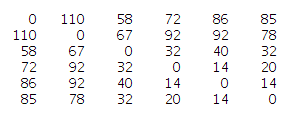
\includegraphics[width=.8\linewidth]{mds_example_input_matrix}
        \caption{Distance matrix input to MDS}
    \end{subfigure}
    \begin{subfigure}{.5\textwidth}
        \centering
        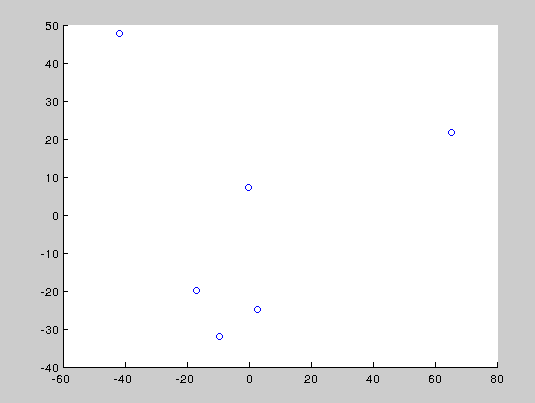
\includegraphics[width=.8\linewidth]{mds_example_output_plot}
        \caption{Output of MDS}
    \end{subfigure}

    \caption{An example of multidimensional scaling showing the input distance
    matrix and the resulting points}
    \label{fig:mdsexample}
\end{figure}


The paper \citep{Qian2004} may seem to imply that this 
transformation is unnecessary since their conclusion is that in high-dimensional 
spaces, the cosine and Euclidean distances can be used interchangeably with 
little difference. However, they note that the similarity of the two measures 
peaks near 32 and then starts slowly 
descending. The highest number of dimensions they examine in their paper is 128. 
However, the vectors generated by my skip-gram model are 800-dimensional 
vectors. Even with a slow descent there is room for the two measures to have 
diverged significantly in a span 8 times the range of the original study. I 
confirmed my suspicions by manually examining 10 randomly chosen words. When 
using the 20 nearest neighbors under the Euclidean distance, the closest 2 or 3 
seemed highly relevant. However, when using the cosine distance, 5-10 seemed 
highly relevant. Thus, for my data set, the difference between the cosine and 
Euclidean distance seems important. 

\section{PCA}

Once the vectors were rearranged in a Euclidean topology, I could perform PCA. 
I performed PCA in two ways, both using the princomp tool in Matlab \todo{ref 
matlab citation}\footnote{Any other tool (R for example) would give the same 
results}. The first was the standard, mean-centered rotation where I subtracted 
the column mean from each dimension in the meaning vectors before extracting the 
components. The second way both subtracted the mean and divided the columns by 
their standard deviation before performing the rotation. This second way is 
similar to the approach taken in exploratory factor analysis. 

I used two approaches because they will bring out components based on different 
criteria and both criteria might be relevant in my domain. The mean-centered 
version attaches importance to the scale of a variable. If variable x is always 
10 times greater than y, a principal component will align more with x than with 
y. When the variables are divided by their standard 
deviation, the variability in an individual variable is canceled out. Then the 
principal components reflect the correlation structure of the system. If x and y 
covary strongly, a principal component will tend to align with the axis of their 
common variability.

\section{Choosing Elbows}

PCA rotates the dataset so that the direction which captures the most
variance is the first axis and all other axes are chosen to capture
the most remaining variance. These axes are the principal components
of the data. One does PCA because one believes that the experimental
manipulations whose effects one seek to capture should be the source
of most of the variance in the data. The rest of the variance in the
data generated by processes not of interest to the current
investigation. Since, in a well controlled experiment, the variation
produced as a result of experimental manipulation is significantly
greater than the variation from other sources, one can identify the
components associated with experimental variation by looking at those
which capture a much larger portion of the total variation than their
fellows\footnote{Assuming a roughly linear response of measured
  components to the underlying variables.}. In general, an effective
way of detecting these components is hand-analysis of a
scree-plot\footnote{A scree plot plots the component index in the
  horizontal axis and the corresponding eigenvalue (corresponding to
  the proportion of variance accounted for) on the vertical axis},
looking for where the slope changes from steeply decreasing to
shallowly decreasing. Although subjective, in Monte Carlo studies this
``Scree test'' identifies the correct number of factors 42\% of the
time. \todo{ref Zwick \& Velicer 1986 ``Comparison of five rules for
  determining the number of components to retain'' Psychological
  Bulletin, 99, 432-442}.

To help guide my intuition, I also threw together a few ad-hoc algorithms that 
did what I thought I was doing in choosing the number of factors. I called 
these algorithms, \filename{elbow\_point}, \filename{flex\_end\_elbow\_point}, 
\filename{offset\_elbow\_point}, \filename{log\_scree\_elbow}, and 
\filename{scree\_elbow\_using\_robust\_fit}. The details of these algorithms can 
be found in \ref{app:elbow_point_algorithms}. But the general ideas behind them 
are simple. They are based off of two conceptions of what humans do in selecting 
the separating line in a scree plot. First, humans try to look for where the 
graph looks like the slope changes abruptly. Second, humans try to look for the 
left-most point where the graph ceases to appear as an exponential decay.

By choosing numbers of components that match human intuition and also
examining points suggested by the heuristic algorithms, I can come up
with a good guess as to how many components I might need to examine.

I entered this experiment assuming a basically linear underlying
structure because such a structure exists in the normal personality
assay manner of determining personality components. However, the scree
plots I generated bear a broad resemblance to those in \todo{cite my
  blog post on the shifted 1's problem} where a nonlinear structure
made the basic elbow method and the other heuristics I used perform
poorly in determining the number of components (the correct number of
components was much greater than any number chosen by any of the
heuristics).

Because of the strong possibility of nonlinear structure, the number
of components I examined depended mostly on my time rather than
criteria in the data. In general I only examined the first 15
principal components of any transformed dataset.

\section{Sorting words to identify components}

With components chosen, the next 
step is to identify the meaning associated with each component if I can. This 
step is necessary to test the hypothesis that the same dimensions show up in 
word meaning as show up in describing individual personality. For each 
principal 
component, I sorted the words by each word's score on that component. Then I 
listed, in order, the 30 highest and lowest scoring words for each dimension. 
The intuition is that if a semantic dimension corresponds to some known 
personality dimension, words positively associated with that dimension will 
have 
a high rating and thus appear near the top of the list. On the other hand, 
words 
negatively associated with that dimension will appear near the bottom of the 
list. Words with no association will appear in the middle. Thus, if a dimension 
corresponds to conscientiousness, I expect ``punctual'' and ``orderly'' to 
appear near the top, ``irresponsible'' to appear near the bottom, and ``gregarious''
to appear in the middle.

\section{Matching components}
\label{sec:matchingcomponents}
Since some of the smaller datasets were not easy to interpret by themselves, I
wanted to check whether the components in the more-interpretable larger datasets
matched the components extracted in the smaller datasets or if the two sets
of word-lists were extracting entirely different facets of meaning as
significant.

To compare two components from two different word-lists, I first reduced the
word-lists to only the common words. Then I looked at the correlation between
the scores assigned to words in one list and the words assigned to the other.
Because I do not know the distribution of word scores, it was safer to use
Spearman correlation to determine significance.

Once I had the correlations and the associated p-values between all pairs of
components, I controlled the false discovery rate at 1\% using the procedure
from \todo{ref cite Benjamini, Y. \& Yekutieli, D. (2001) The control of 
the false discovery rate in multiple testing under dependency. 
The Annals of Statistics. 29(4), 1165-1188}. I chose to control false discovery 
rate rather than
family-wise error rate because decisions about this data depend mainly on the
individual component pair matches rather than on the whole collection being 
right or wrong. I used Benjamini and Yekutieli rather than the more common
Benjamini and Hochberg because it is possible that my data violates the 
positive dependence assumption in 
\todo{ref cite Benjamini, Y. \& Hochberg, Y. (1995) Controlling the false 
discovery rate: A practical and powerful approach to multiple testing. Journal
of the Royal Statistical Society, Series B (Methodological). 57(1),
289-300.}. Benjamini and Yekutieli does not have this restriction, thus it was
more appropriate.

Multiple test correction trades off Type I error (false matches in this case) 
for Type II error (missed matches). Because I anticipated that most matches
would be in the first components and because I wanted to have as few missed
matches as possible, I used a sequential procedure to choose which dimensions
to compare based on matches in other datasets.

I started by comparing all components of the 2797 word set with all 
components from the combined 101 and 438 word sets. I then chose a number of
dimensions that got the vast majority of matches (possibly excluding a few
outliers). For the MDS transformed data, this was the first 52 components. 
Then, I compared the 101 and 438 word sets on only these dimensions. Again I
selected the number of components that best captured the matches. Finally,
I compared the 101 and 2797 word sets on the number of dimensions derived from
the 101 and 438 word comparison. 

This procedure makes the test less likely to miss matches in the region most
likely to contain them by ignoring potential matches in the other regions.

\end{document}
